\documentclass[11pt]{article} % use larger type; default would be 10pt

\usepackage{algpseudocode}
\usepackage{mathtools}

\usepackage[utf8x]{inputenc} % set input encoding (not needed with XeLaTeX)

%%% Examples of Article customizations
% These packages are optional, depending whether you want the features they provide.
% See the LaTeX Companion or other references for full information.

%%% PAGE DIMENSIONS
\usepackage{geometry} % to change the page dimensions
\geometry{a4paper}

\usepackage{graphicx} % support the \includegraphics command and options

% \usepackage[parfill]{parskip} % Activate to begin paragraphs with an empty line rather than an indent

%%% PACKAGES
\usepackage{booktabs} % for much better looking tables
\usepackage{array} % for better arrays (eg matrices) in maths
\usepackage{paralist} % very flexible & customisable lists (eg. enumerate/itemize, etc.)
\usepackage{verbatim} % adds environment for commenting out blocks of text & for better verbatim
\usepackage{subfig} % make it possible to include more than one captioned figure/table in a single float
% These packages are all incorporated in the memoir class to one degree or another...

%%% HEADERS & FOOTERS
\usepackage{fancyhdr} % This should be set AFTER setting up the page geometry
\pagestyle{fancy} % options: empty , plain , fancy
\renewcommand{\headrulewidth}{0pt} % customise the layout...
\lhead{}\chead{}\rhead{}
\lfoot{}\cfoot{\thepage}\rfoot{}

%%% SECTION TITLE APPEARANCE
\usepackage{sectsty}
\allsectionsfont{\sffamily\mdseries\upshape} % (See the fntguide.pdf for font help)
% (This matches ConTeXt defaults)

%%% ToC (table of contents) APPEARANCE
\usepackage[nottoc,notlof,notlot]{tocbibind} % Put the bibliography in the ToC
\usepackage[titles,subfigure]{tocloft} % Alter the style of the Table of Contents
\renewcommand{\cftsecfont}{\rmfamily\mdseries\upshape}
\renewcommand{\cftsecpagefont}{\rmfamily\mdseries\upshape} % No bold!
%%% END Article customizations

%%% The "real" document content comes below...
\title{Brief Article}
\author{The Author}
%\date{} % Activate to display a given date or no date (if empty),
         % otherwise the current date is printed

\begin{document}
\maketitle

\abstract{THIS IS THE ABSTRACT}

\subsubsection*{Keywords}
graph, triangles count


\label{Introduction}
\section{Introduction}

The IMDB dataset provides data about actors, movies and relations between them. Based on this dataset a number of interesting properties can be extracted from the data. The point, however, is doing this in efficient manner.
\\
\\
In section \ref{ProblemDescription} we examine the problem, its input and expected output. In section \ref{MisraGries} we look at a standard approach for solving the problem - using the well known Misra-Gries streaming algorithm. We present the running time and space usage for various input sizes. In the next section we turn our attention to our algorithm that improves on many of shortcomings of Misra-Gries. Further section \ref{Parallelism} explores a way of improving our algorithm running time by running it in parallel. In section \ref{Experiments}, we present results of experiments we conducted on IMDB database.


\label{sec:ProblemDescription}
\section{Problem Description}

The \textbf{goal} is to find the three actors, whose movie count they have played together in is maximized among he whole dataset.

\textbf{Input} is a list of actors, movies and actor-movie pair, for each actor that has played in a movie.

\textbf{Output} is a list of actors with the desired property, on an empty list if no three actors have played together in the same movie.


\label{Algorithm}
\section{Algorithm}

The algorithm we are presenting works on two main steps:
\begin{itemize}
  \item Build the data structure - the efficiency of the algorithm is determined by the data structure it runs on. On the other hand, the data structure is specifically designed to solve this problem.
  \item Traverse data structure and output result - the algorithm works by looping through all the actors and finding the most promising connections.
\end{itemize} 

\subsection{Notations}
Let G = (V,E) be a weighted, directed simple graph and let n = \(\lvert V\rvert\) and m = \(\lvert E\rvert\).

A vertex v denotes an actor. Any edge e between vertices \(v_1\) and \(v_2\) denotes a set of movies these two actors have played together. Weight of the edge, W(e) denotes the size of that set. An edge is always directed from the actor with lower Id to the actor with higher Id.

Denote by A(v) the set of adjacent edges to vertex v.

SET(e) is the set of (two) vertices adjacent to an edge e.

Unique(\(v_1, v_2,... v_n)\) - returns a set of unique elements.

MovieCount denotes the biggest number found so far of common movies between any given three actors.

\subsection{Data structure}
As mentioned in the previous section, the algorithm starts by first building the data structure. The data structure is a graph, where vertices represent actors and edges between them represent the movie(s) these actors played together in. 

\begin{figure}[ht!]
\centering
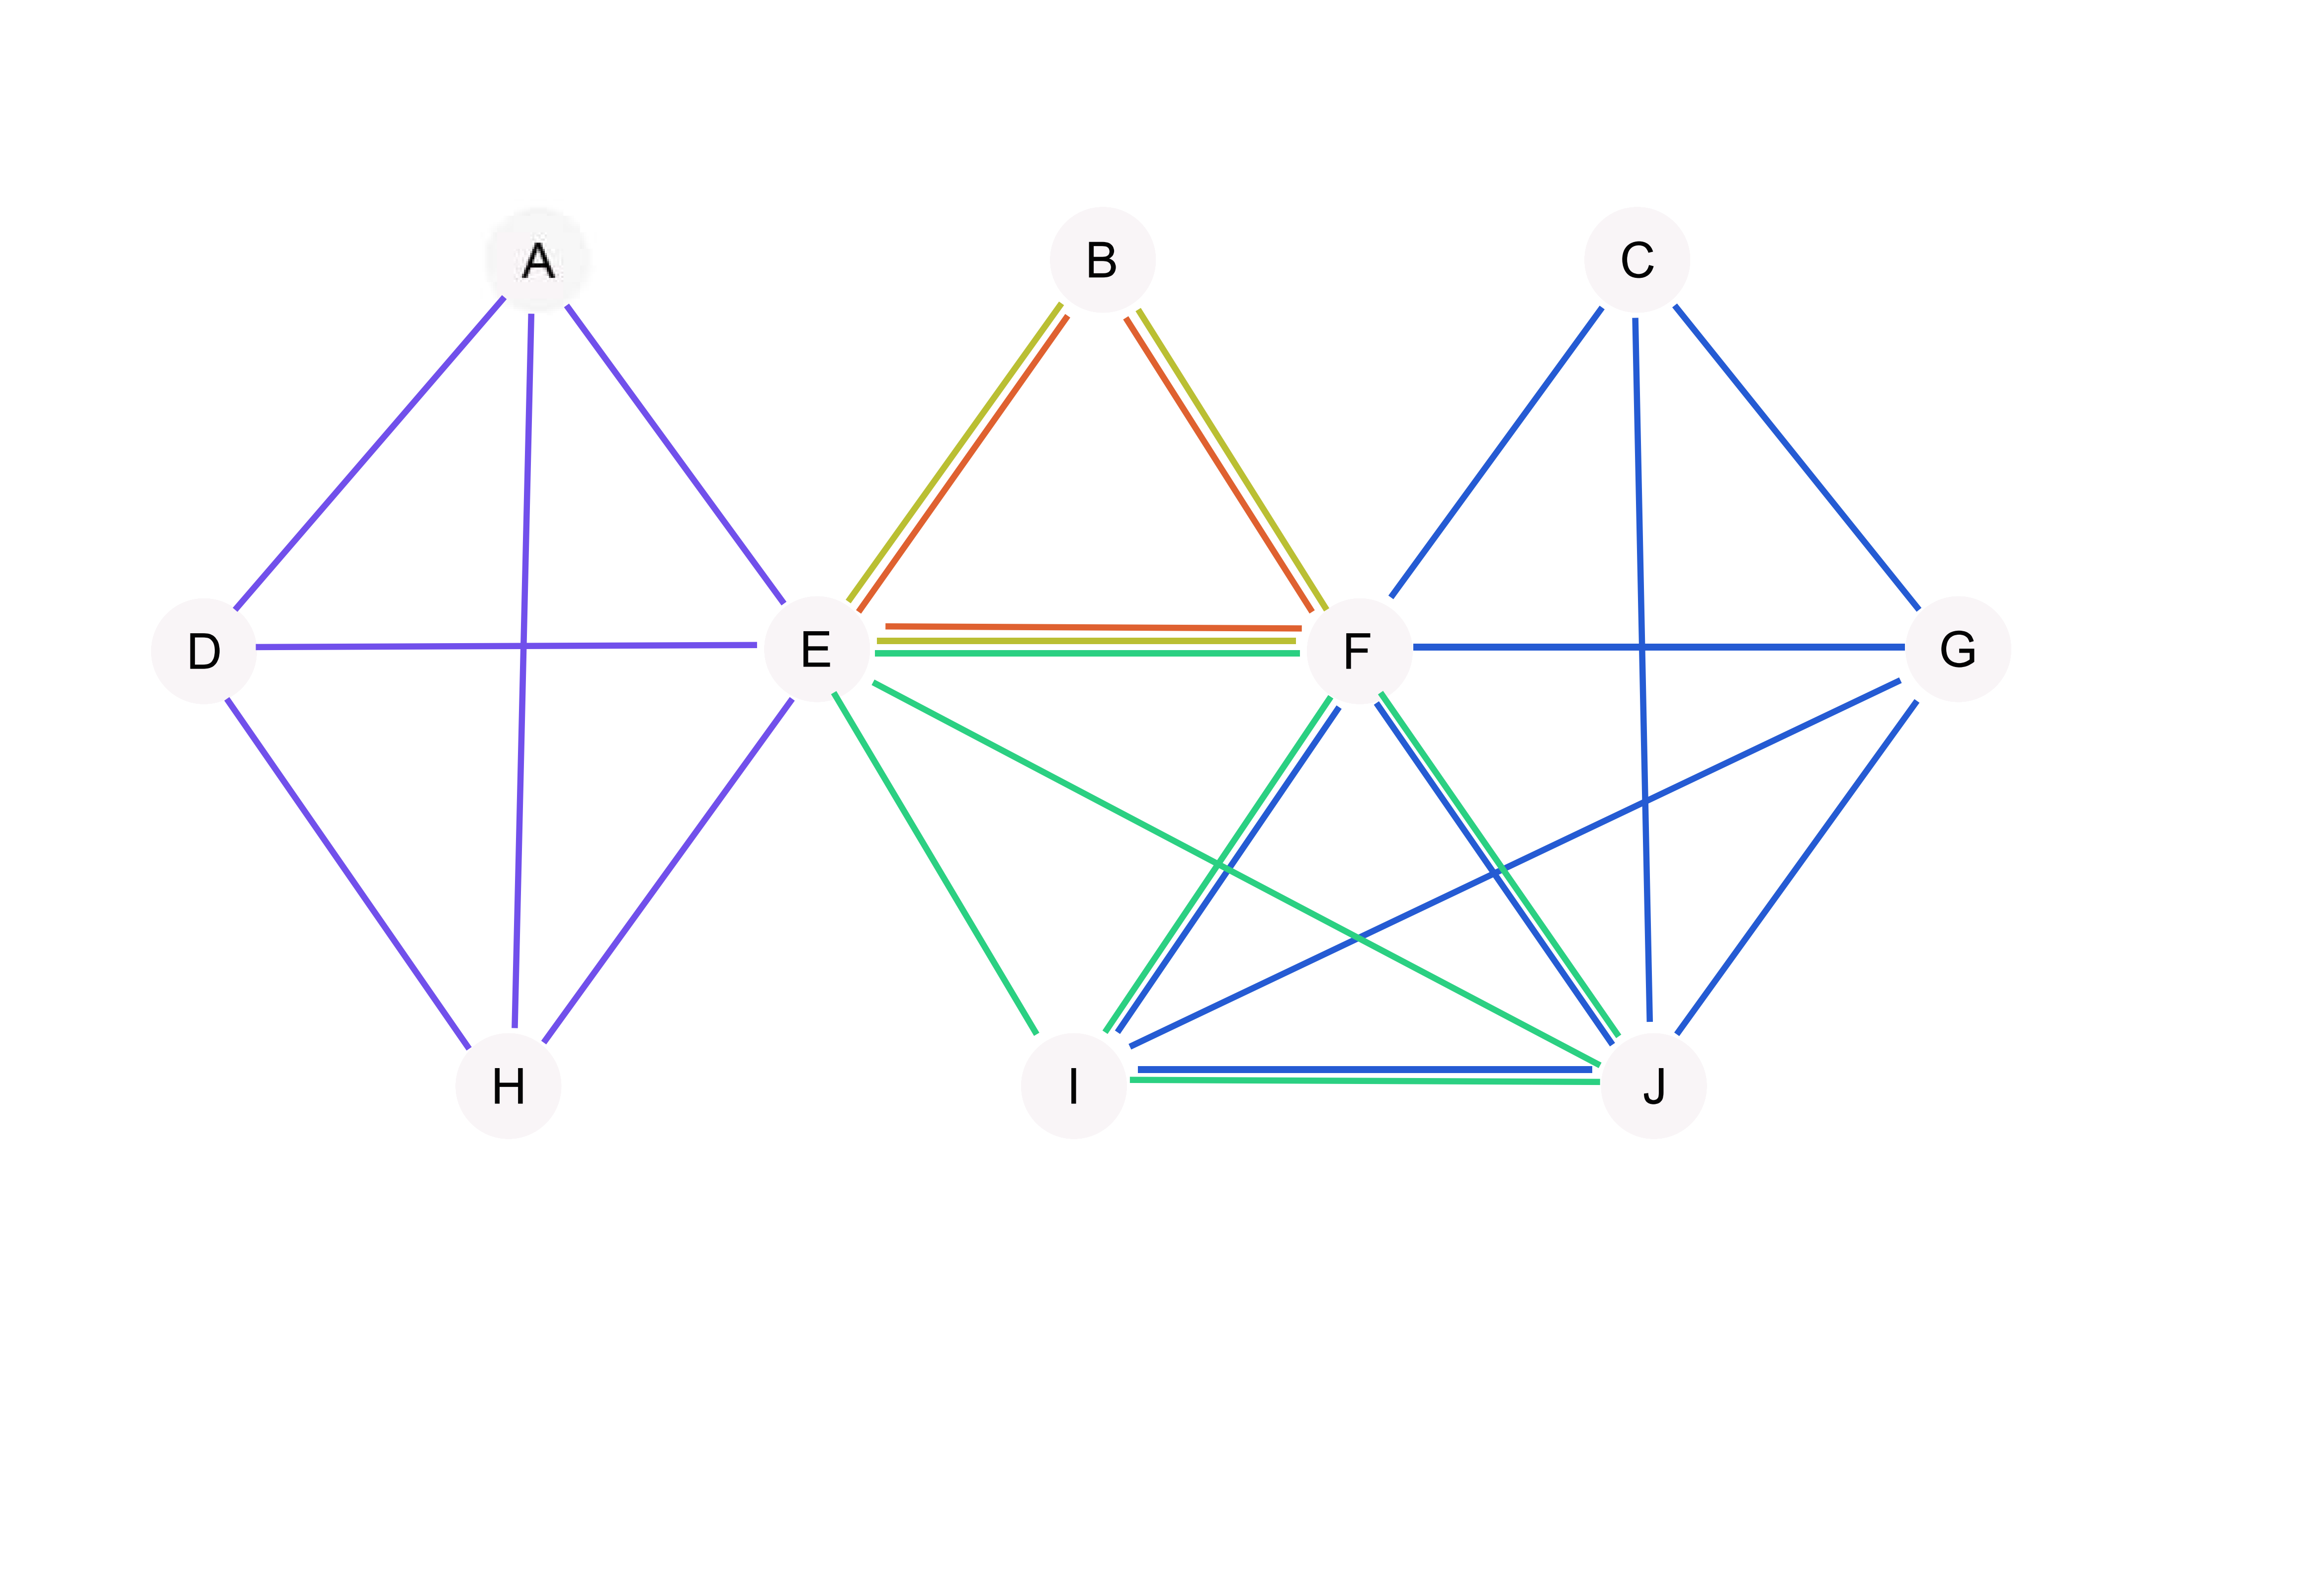
\includegraphics[width=130mm]{resources/project_problem_illustration.png}
\caption{Graph Example}
\label{example}
\end{figure}

Figure \ref{example} represents the data structure. To clearly illustrate the problem, the picture above represents a multi-graph, i.e. there can be multiple edges between two vertices. This is not the case of the actual data structure, however, as multiple edges are collapsed into a single one, where the weight is the sum of the weights of the original edges. The weight of an edge is the initially 1 - a single movie common to two actors (vertices). The edge contains sorted list of the movies common for two actors adjacent to the specific edge.
\\
After the structure is constructed, the actual data processing takes place.


\subsection{Pseudocode}
Main algorithm we implemented is FindThreeActors. After constructing the graph, we iterate over all vertices (actors). We find for each vertex all subsets of size of two of the set of adjacent edges to that vertex. We take an advantage of the fact that if an actor 1 played together in the same movie "A" with an actor 2 and the actor 1 played together with an actor 3 in the movie "A", that means that the actor 2 and the actor 3 had to play together in the movie "A". So we decided not to look for triangles in traditional way, but we look for pairs of edges having movies in common being adjacent to a specific vertex.
\\
We examine each pair of edges and we find the number of common movies that actors played in together (this is a common set of the subsets - the movies from two edges).  We do that only if minimal weight of edges is higher than found (by now) maximum number of movies that actors played together. 
\\
If the solution is better that the already found, we save it. We continue searching and at the end, we remove any references to the adjacent edges to the analysed vertex. This will make future iterations faster, since less edges need to be examined. We go to the next iteration. 
\\
Pseudocode for the algorithm is presented below:

\begin{verbatim}
Algorithm 2: FindThreeActors(graph)
1	moviesCount ← 0;
2	{a1,a2,a3};
3	FOR v ∈ V DO
4	  FOR i ← 0 to size of A(v) DO
5	    e1←A(v)[i];
6	    IF MoviesCount < W(e1) THEN
7	      FOR j ← i + 1 to size of A(v) DO	          
8	          e2←A(v)[j];
9	          IF MoviesCount < W(e2) THEN
10	              count ← CommonMovieSubsetCount(e1, e2);
11	             IF moviesCount < count THEN
12	                  movieCount ← count;
13	                  {a1,a2,a3} ← Unique(SET(e1), SET(e2));
14	             END IF
15	          END IF
16	      END FOR
17	    END IF
18	  END FOR
19	END FOR
20	RETURN moviesCount, {a1,a2,a3};	  	                    	  
\end{verbatim}


We designed CommonMovieSubsetCount that returns number of items that are common in 2 subset given as arguments. We take advantage of the fact that the lists are sorted and we iterate over all the items in both list in linear time. 
\\
The pseudocode is present below:

\begin{verbatim}
Algorithm 3: CommonMovieSubsetCount(movies1, movies2)
1	count ← 0;
2	p1 ← 0;
3	p2 ← 0;
4	WHILE p1 < W(movies1) AND p2 < W(movies2)
5	  IF movies1[p1] = movies2[p2] THEN
6	    INCREMENT(count);
7	    INCREMENT(p1);
8	    INCREMENT(p2);
9	  ELSE IF movies1[p1] < movies2[p2]
10	   INCREMENT(p1);
11	 ELSE IF movies1[p1] > movies2[p2]
12	  INCREMENT(p2);
13	END IF
14	RETURN count;
\end{verbatim}

\subsection{Parallelism}
Since the IMDB database is enormous and building graph for such an amount of data, requires lots of RAM, we wanted to split the problem and make computations on separate parts in parallel. We took care of not loosing any data and not processing any data more times than once. The other important thing was to split data into parts that require the same amount of work for CPU.
\\
Each separate group contains specific number of actors and edges coming out from them. The division is done by creating a list of edges (an edge contains 2 actors and a movie these 2 actors played together), where there is no repetition of edges (an edge is always directed from an actor with higher Id to an actor with lower Id). We sorted the list according to the Id of the first actor (in this actor with lower Id in an edge). We noticed that since an edge goes to the actor with higher Id, vertices with lower Ids have much more edges going out from it than getting in, so we could not just picked the first x actors from the list. To split data evenly, we just picked every ???? actor from the sorted list we have. That guaranties that workload on every part of data is similar.
\\
We claim that we have no repetition of processing data. It is shown on the picture below....
All three vertices are connected to each other and we put them in three different groups (red, blue and green). In group red we have a vertex A and two edges coming out from this vertex. In blue group we have a vertex B and one edge coming out from it. In group green we have only vertex C without any edges. We can see that the presented triple will be analysed only once when we will process the vertex A in group red.
\\
The presented division allows us to run computations in parallel. Each thread results in a triplet and number of movies actors played together. After finishing computing all the data, we just need to aggregate the results and find the triplet that played in the most number of movies. The picture !!!!!
\\

\subsection{Analysis}
By not choosing to implement a traditional triangles counting, we avoided to examine three times the same triple of the actors and the number of their common movies thay played in. To be able to avoid this, we constructed a special data structure and by consolidating edges, we saved used space to save the data.
In the worst case scenario, when each actor played together with another one (it is not realistic situation though) we will have n vertices and n*(n - 1)/2 edges.
\\
Complexity of the algorithm highly depends on degree of vertices. The higher it is, the longer computation time is needed. It is related to the process of looking for subsets of size two for each vertex. The complexity of the algorithm is \(\sum\limits_{i=1}^n{k_i \choose 2}\) where \(k_i\) is size of A(\(v_i)\), v \(\in\) V, which we can reduce to \(\sum\limits_{i=1}^n{k_i^2}\).
\\
Comparison with Misra-Gries...

\input{./Analysis.tex}
\section{Conclusion}
\label{Conclusion}

While a streaming algorithm as Misra-Gries provides the advantage of less memory usage, it has one key disadvantage for our problem - the need to explore every possible triplet combination. In cases where the actors count of a movie is too big (1000+), this introduces an unacceptable running time. Our approach goes away with this by managing to explore a triplet only once. Furthermore, it allows for parallelisation of the computation by allowing subsets of the data to be computed independently.


\subsection{Future Work}
Possible future work might be exploring counting triangles algorithm. We can build graph in the same way we presented, but we analyze each triangle in the graph instead (a triangle represents a triplet of actors). Counting triangles method using MapReduce gives good results and might be an interesting alternative to our approach \footnote{http://theory.stanford.edu/~sergei/papers/www11-triangles.pdf}.
\label{References}\section{References}

\end{document}
